\section{Epipolar Geometry}

\textbf{这一章节在教学中已经被删去,为了让有兴趣的读者了解,故保留}

\begin{wrapfigure}{r}{4cm}
	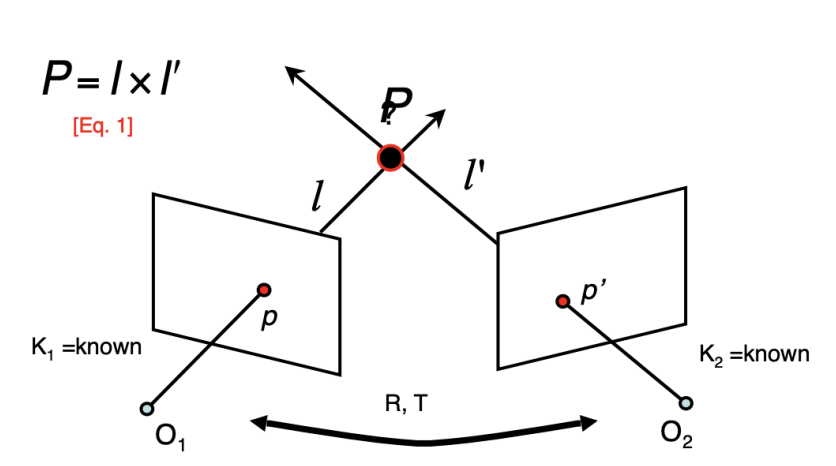
\includegraphics[scale=0.3]{figures/triangulation.png}
	\caption{Triangulation}
\end{wrapfigure}

既然单个视角无法确定深度,那么我们自然会想到如果有多台相机或许就可以确定距离,如同人眼一样.

原则上,两台相机就可以确定点的位置.我们看右图:$O_1, O_2$代表两台相机的镜心,两个平行四边形代表各自的像平面,如果一个点$P$在两个像平面的投影点$p, p^\prime$已知,我们就可以确定$P$点在镜心到对应点的连线交点的位置.

在前面的章节当中我们已经介绍了校准相机的方法,而两台相机的位置参数$\bd R, \bm t$一般都是已知的,此时的关键问题就是:\textbf{确定一个点在另一个相机图片的位置}.



\begin{figure}[htbp]
	\centering
	\subfigure[对极几何中的基本概念]{
		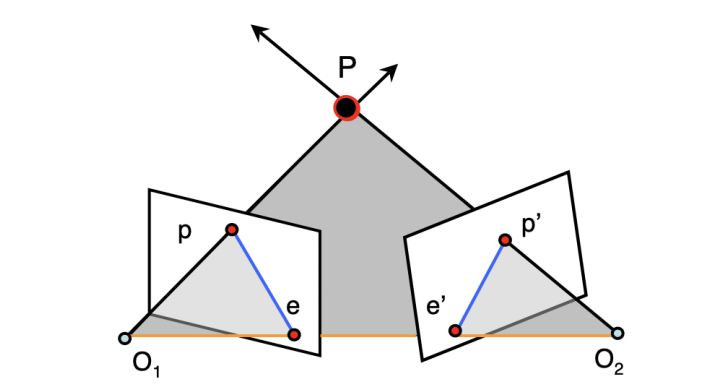
\includegraphics[scale=0.45]{figures/epipolargeometry.png}
	}
	\subfigure[像平面平行的情形]{
		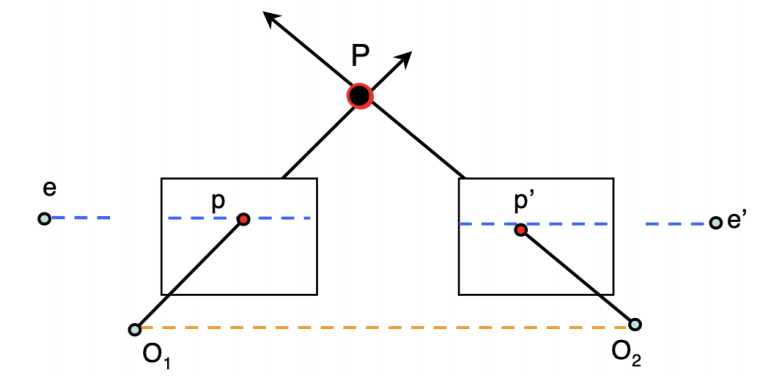
\includegraphics[scale=0.45]{figures/parallel-image-plane.png}
	}
\end{figure}

与这一任务相关的几何内容被称为对极几何(epipolar geometry).我们先给出对极几何当中的一些概念.

左图中由$O_1, O_2, P$三点构成的平面(图中灰色填充)被称为epipolar plane.连线$O_1O_2$被称为baseline.baseline与两个像平面的交点被称为epipole.各个像平面内,epipole与$P$的投影点被称为epipolar line.

当$P$点移动时,相当于极平面上下翻动,此时对应的极线也会变化,但是所有的极线都通过极点.

一种特殊情况是两个像平面相互平行,此时极点位于无穷远处,图中所有极线都平行于基线.
那么,给定图片中的一个点,要如何去确定在另一张图片中这个点的对应呢?我们看下图,根据给定点和基线我们可以确定极平面,极平面与右像平面的交点即为极线,对应点$p^\prime$必定在此极线上,也就将对应点的搜索从2维降低到了1维.
\begin{figure}[htbp]
	\centering
	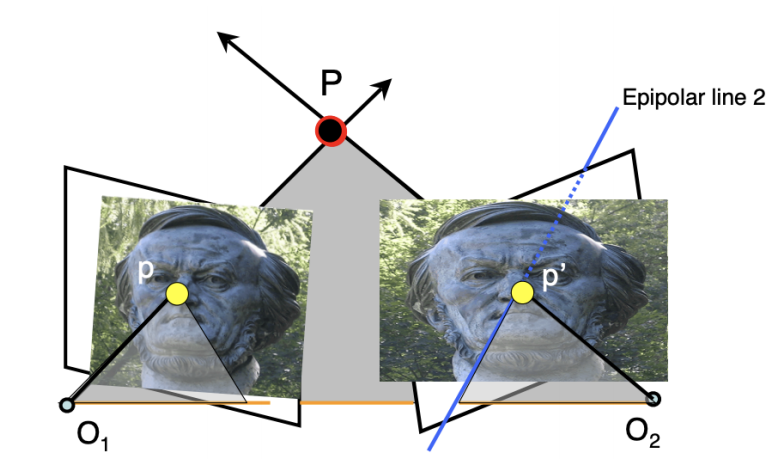
\includegraphics[scale=0.45]{figures/epi-geo-2pic.png}
	\caption{两张图片的对应}
\end{figure}

\subsection{Epipolar Constrain}
首先我们先确定两台相机的位置.如下图,方便起见,假设世界坐标与第一台相机的坐标重合,第二台相机的坐标系由旋转$\bd R$和偏置$\bm t$确定.对于一点$\bm P$,如果它在两台相机的坐标系下的坐标分别是$\bm p_E, \bm q_E$,则有关系
\begin{equation}
	\bm q_E = \bd R^{\top}\xk{\bm p_E - \bm t}
\end{equation}

因此,两台相机的变换矩阵分别是
\begin{equation}
	\bd M = \bd K
	\begin{bmatrix}
		\bd I & \bm 0
	\end{bmatrix} ,
	\quad
	\bd M^\prime = \bd K^\prime
	\begin{bmatrix}
		\bd R^{\top} & \bm -\bd R^{\top} \bm t
	\end{bmatrix}
\end{equation}


\begin{figure}[htbp]
	\centering
	\subfigure[两台相机的位置]{
		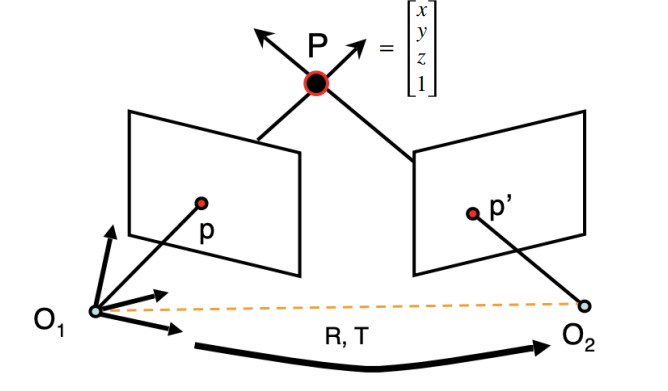
\includegraphics[scale=0.45]{figures/epi-constrain.png}
	}
	\subfigure[坐标变换]{
		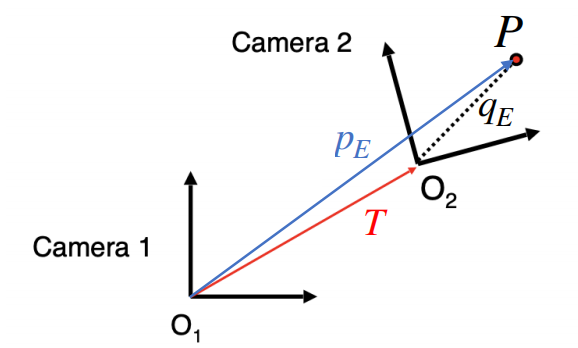
\includegraphics[scale=0.45]{figures/camata-pose.png}
	}
	\subfigure[对极约束]{
		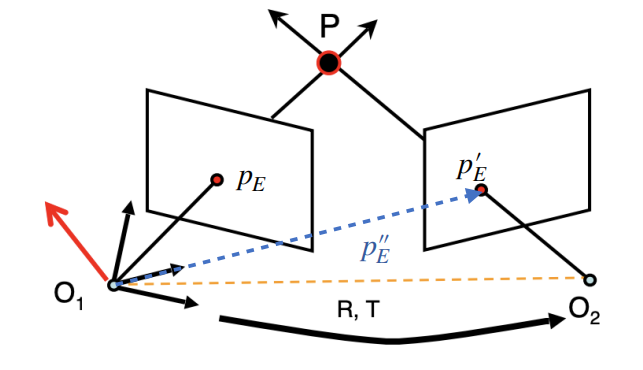
\includegraphics[scale=0.45]{figures/epi-constrain-2.png}
		\label{fig:epi-constrain-2}
	}
	\caption{}
\end{figure}

如图 \ref{fig:epi-constrain-2} ,我们规定以下符号:$\bm p_E, \bm p_E^\prime, \bm p_E^{\prime\prime} \in \mathbb R^3$分别代表左投影点在左相机坐标系(即世界坐标系)的坐标,右投影点在右相机坐标系下的坐标,右投影点在左相机坐标系下的坐标.我们可以求出极平面的法向量(图中红色箭头):
\begin{equation}
	\bm n = \bm t \times \bm p_E^{\prime\prime} = \bm t \times \xk{\bd R \bm p_E^{\prime} + \bm t} = \bm t \times \bd R \bm p_E^{\prime}
\end{equation}

对于两个向量$\bm a = [a_x, a_y, a_z]^\top, \bm b = [b_x, b_y, b_z]^\top$的叉乘,可以表示成矩阵形式:
\begin{equation}
	\bm a \times \bm b  = \zk{\bm a_{\times}}\bm b = 
	\begin{bmatrix}
		0 & - a_z & a_y
		\\
		a_z & 0 & -a_x
		\\
		-a_y & a_x & 0
	\end{bmatrix}
	\begin{bmatrix}
		b_x
		\\
		b_y
		\\
		b_z
	\end{bmatrix}
\end{equation}
不难看出这是一个反对称矩阵,秩为$2$.

显然有$\bm p_E \perp \bm n$,写成矩阵形式就是

\begin{equation}
	\bm p_E^\top \zk{\bm t_{\times}}\bm R \bm p^{\prime}_E = 0
	\label{eq:essential-matrix}
\end{equation}

我们定义
\begin{equation}
	\bd E = \zk{\bm t_{\times}}\bm R
\end{equation}
为本质矩阵(essential matrix).它是一个形状为$3 \times 3$,秩为$2$的矩阵,有五个自由度.\footnote{在下文的基本矩阵的讨论中,我们也会涉及到自由度的问题,这一度令笔者陷入困惑.这些内容将在附录 \ref{DOFandRank} 当中作进一步探讨.}

代入式 \ref{eq:essential-matrix}得到:
\begin{equation}
	\bm p_E^\top \bd E \bm p^{\prime}_E = 0
\end{equation}

虽然有了本质矩阵是在两个相机坐标系下的三维坐标的变换,我们自然希望能用二维的图片坐标进行直接对应.考虑到
\begin{equation}
	\bm p_E = \bd K^{-1} \bm p, \quad \bm p_E^\prime = \bd K^{\prime-1} \bm p^\prime
\end{equation}

代入式 \ref{eq:essential-matrix}即得
\begin{equation}
	\bm p^\top \bd K^{-\top} \zk{\bm t_{\times}}\bd R \bd K^{\prime-1} \bm p^{\prime} = 0
\end{equation}

我们定义
\begin{equation}
	\bd F = \bd K^{-\top} \bd E \bd K^{\prime-1} = \bd K^{-\top} \zk{\bm t_{\times}}\bd R \bd K^{\prime-1}
	\label{eq:fundamental-matrix}
\end{equation}
为基本矩阵(fundamental matrix),它是一个秩为$2$,自由度为$7$的$3 \times 3$矩阵.式 \ref{eq:fundamental-matrix}变为
\begin{equation}
	\bm p^\top \bd F \bm p^{\prime} = 0
	\label{eq:fundamental-mat}
\end{equation}


\begin{wrapfigure}{r}{6cm}
	\centering
	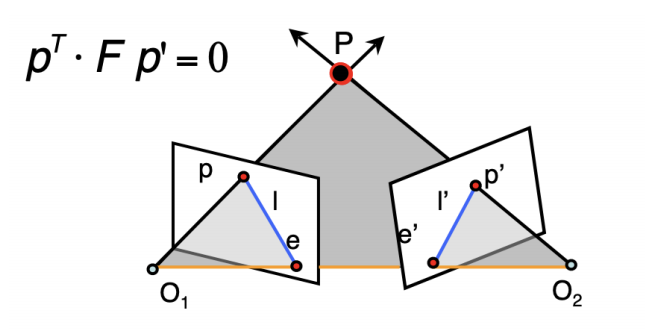
\includegraphics[scale=0.55]{figures/property-of-f-mat.png}
	\caption{基本矩阵的性质}
	\label{fig:property of fundamental matrix}
\end{wrapfigure}

除此之外,基本矩阵还有如下性质:如图 \ref{fig:property of fundamental matrix},首先,$l = \bd F \bm p^\prime$和$l^\prime = \bd F^{\top} \bm p$分别是$\bm p, \bm p^\prime$对应的极线.其次,$\bd F \bm e^\prime = 0, \bd F^\top \bm e = 0.$

先证明前者.式 \ref{eq:fundamental-mat}说明$\bm p \in l$.设$\bm e$对应的世界坐标为$\bm e_E$,则由于$\bm e_E \perp \bm n$,因此式 \ref{eq:essential-matrix}及以后的各式将$\bm p_E$替换成$\bm e_E$都成立,那么同式 \ref{eq:fundamental-mat}的形式,我们亦可以得到

\begin{equation}
	\bm e^\top \bd F \bm p^{\prime} = 0.
	\label{eq:all points in epipolar plane}
\end{equation}

由此得出$\bm e \in l$.\footnote{细心的读者不难发现,极平面内所有的点都可以这样做,而这个结论也是非常自然的,因为极线正是极平面射影在左像平面的结果.}

对于后者,我们知道$\forall \bm p$,都有式 \ref{eq:all points in epipolar plane}成立,因此只能有
\begin{equation}
	\bd F \bm e^\prime = 0, \quad \bd F^\top \bm e = 0.
\end{equation}

我们对本质矩阵和基本矩阵做一个总结.

$\bd E$是两个标准相机相对关系的内参,换言之,给定两个已标定相机的相对位置关系,$\bd E$即被确定.

$\bd F$是任意两个相机相对关系的内参,换言之,给定了两个相机的相对位置关系和相机内参,$\bd F$即被确定.

如果我们能够求出$\bd F$,那么就可以在不进行三维重建的情况下,确定两张照片的对应关系.还记得我们在上节末尾和这节的开头提出的问题吗?在上一节的末尾,我们说通过两台相机即可确定深度信息,在这一节的开头我们引入了对极几何的概念,我们的目的是确定两张照片中的对应点,再通过两台相机的方向即可求出点的深度,而方向已经在上一节中解决.现在我们离解决这个问题只剩最后一步,即如何求出$\bd F$?

我们设$\bd F = (F_{ij})$,根据式 \ref{eq:fundamental-mat},如果有8对对应点\footnote{这里读者可能会产生一个问题,既然$\bd F$的自由度为$7$,为什么要8对对应点呢?其中原因之一是,相机的内部性质多为非线性,所以使用最小点数求解可能会比较麻烦,因此经常只考虑尺度的等价性,忽略奇异性条件,此时自由度为8.}的坐标$(u_i, v_i, 1)^{\top} \leftrightarrow (u_i^\prime, v_i^\prime, 1)^{\top}$, 那么我们可以得到方程组
\begin{equation}
	\begin{pmatrix}
		u_{1} u_{1}^{\prime} & u_{1} v_{1}^{\prime} & u_{1} & v_{1} u_{1}^{\prime} & v_{1} v_{1}^{\prime} & v_{1} & u_{1}^{\prime} & v_{1}^{\prime} & 1 \\
		u_{2} u_{2}^{\prime} & u_{2} v_{2}^{\prime} & u_{2} & v_{2} u_{2}^{\prime} & v_{2} v_{2}^{\prime} & v_{2} & u_{2}^{\prime} & v_{2}^{\prime} & 1 \\
		u_{3} u_{3}^{\prime} & u_{3} v_{3}^{\prime} & u_{3} & v_{3} u_{3}^{\prime} & v_{3} v_{3}^{\prime} & v_{3} & u_{3}^{\prime} & v_{3}^{\prime} & 1 \\
		u_{4} u_{4}^{\prime} & u_{4} v_{4}^{\prime} & u_{4} & v_{4} u_{4}^{\prime} & v_{4} v_{4}^{\prime} & v_{4} & u_{4}^{\prime} & v_{4}^{\prime} & 1 \\
		u_{5} u_{5}^{\prime} & u_{5} v_{5}^{\prime} & u_{5} & v_{5} u_{5}^{\prime} & v_{5} v_{5}^{\prime} & v_{5} & u_{5}^{\prime} & v_{5}^{\prime} & 1 \\
		u_{6} u_{6}^{\prime} & u_{6} v_{6}^{\prime} & u_{6} & v_{6} u_{6}^{\prime} & v_{6} v_{6}^{\prime} & v_{6} & u_{6}^{\prime} & v_{6}^{\prime} & 1 \\
		u_{7} u_{7}^{\prime} & u_{7} v_{7}^{\prime} & u_{7} & v_{7} u_{7}^{\prime} & v_{7} v_{7}^{\prime} & v_{7} & u_{7}^{\prime} & v_{7}^{\prime} & 1 \\
		u_{8} u_{8}^{\prime} & u_{8} v_{8}^{\prime} & u_{8} & v_{8} u_{8}^{\prime} & v_{8} v_{8}^{\prime} & v_{8} & u_{8}^{\prime} & v_{8}^{\prime} & 1
	\end{pmatrix}
	\begin{pmatrix}
		F_{11} \\
		F_{12} \\
		F_{13} \\
		F_{21} \\
		F_{22} \\
		F_{23} \\
		F_{31} \\
		F_{32} \\
		F_{33}
	\end{pmatrix}
	= \bm 0
	\label{eq:8 points to solve F}
\end{equation}

我们记上式为
\begin{equation}
	\bd W \bm f = \bm 0
\end{equation}

如果$\text{rank}(\bd W) = 8$,则$\bm{f}$有唯一非零解.当对应点对数目多于$8$个,则限制$\norm{\bm f} = 1$,使用SVD求解.但是$\bd F$的秩为$2$,那么问题转化为
\begin{equation}
	\begin{aligned}
		\text{minimize } &\norm{\bd F - \hat{\bd F}}
		\\
		\st &  \det{\bd F} = 0.
	\end{aligned}
\end{equation}

而SVD告诉我们,设$\text{rank}(\bd F) = r,$若将$\bd F$按奇异值降序分解为
\begin{equation}
	\bd F = \sum_{i=1}^{r} \sigma_i \bm u_i \bm v_i^\top
\end{equation}

则在所有秩不大于$k$的矩阵当中,
\begin{equation}
	\bd F = \sum_{i=1}^{k} \sigma_i \bm u_i \bm v_i^\top
\end{equation}
就是使得$\norm{\bd F - \hat{\bd F}}$最小的矩阵.因此我们需要对式 \ref{eq:8 points to solve F}求解出的$\bd F$再次进行SVD,并取前两个奇异值和左右奇异向量构成解$\bd{F}$.